\section{Appendix}
\label{section:appendix}

\subsection{CoovaAP}
The CoovaAP setup was fairly straight-forward, if flaky. As mentioned in the proposal, I used a
Linksys WRT54GL \cite{product:WRT54GL} with the corresponding CoovaAP binary, available on their
public website \cite{product:CoovaAPBin}. After the firmware was installed (by using the router's
existing Firmware Update page), I had access to CoovaAP. I found that the Admin page allowing me to
configure the AP was very flaky in Chrome (version TODO) and Firefox (version TODO), but consistent
in Internet Explorer (version 11.0.9600).

Having learned that the Facebook integration is old and no longer works
\cite{article:CoovaFacebookNoMore}, I decided to continue with my original plan of implementing my
own captive portal server.

\subsubsection{Captive Portal Setup}
I managed to find a good tutorial \cite{article:CoovaHotSpotSetup} on setting up a custom captive
portal page and followed it for the following main steps:
\begin{enumerate}
\item{Clear RAM:}  To ensure a fresh configuration, SSH into the router with \texttt{ssh
root@192.168.1.1} (password ``root''), then run \texttt{ mtd erase nvram \&\& reboot }.
\item{Setup Hotspot:}  Back in the Admin page (browse to http://192.168.1.1 in IE), setup a
\texttt{HotSpot Type = Internal Hotspot} with \texttt{Registration Mode = ToS Acceptance} and Save.
\item{Fix Broken Portal:}  In the SSH session, open (with ViM for example)
\texttt{/et c/chilli/www/tos.chi}, then change \textbf{line 37}:
  \begin{enumerate}
  \item{from:} \texttt{ if [ "\$tos" = "1" ]; then }
  \item{to:} \texttt{ if [ "\$HS\_REG\_MODE" = "tos" ]; then}
  \end{enumerate}
\item{Confirm it worked:}  Now try to access the internet via the router (SSID: \texttt{Coova}), you
should see the Terms of Service page with Accept and Decline buttons at the bottom.

\begin{figure}[ht!]
\centering
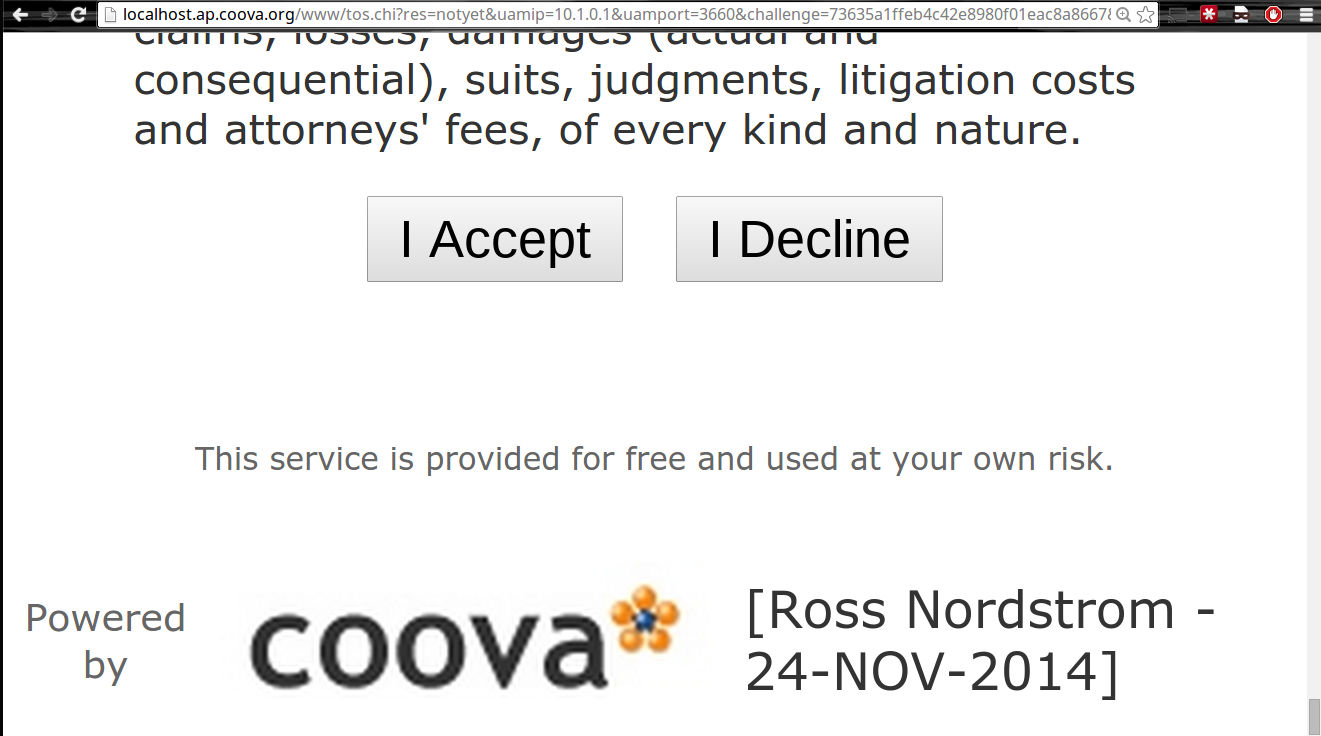
\includegraphics[width=90mm]{fig/footer.png}
\caption{Modified the Captive Portal!}
\label{fig:footer}
\end{figure}

\item{Explore:}  Next I tried to understand how the ToS page was served. Frighteningly, it seems to
be a served up by a Bash script. I managed to find the code driving the Footer and modify it to
include my name \ref{fig:footer}, by modifying a section of
\texttt{/etc/chilli/www/config-local.sh}.

\begin{figure}[ht!]
\centering
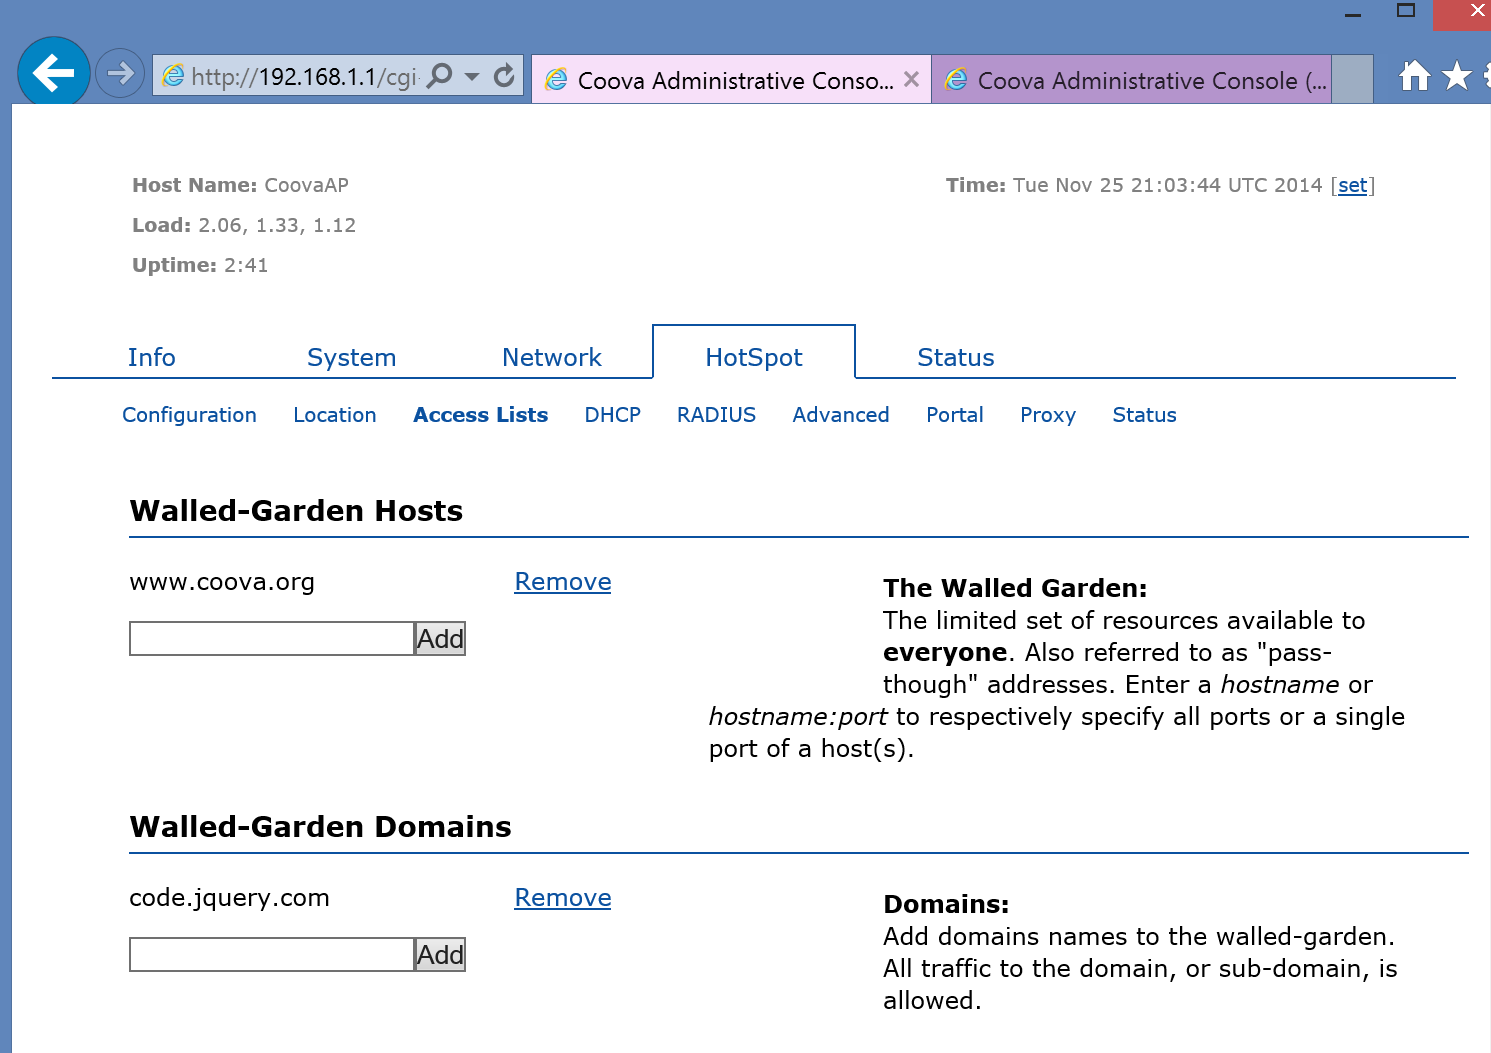
\includegraphics[width=90mm]{fig/allowed_domains1.png}
\caption{Allow jQuery within the Walled Garden}
\label{fig:allow_jquery}
\end{figure}

\begin{figure}[ht!]
\centering
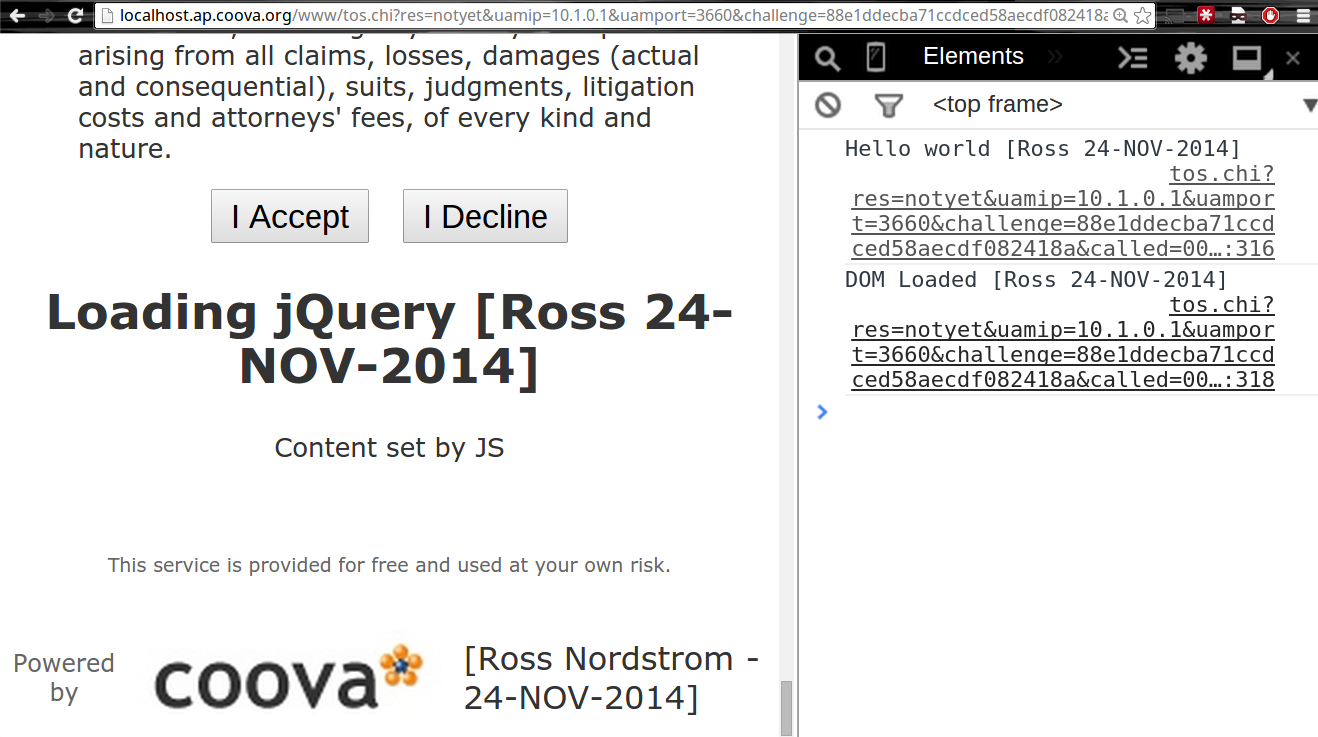
\includegraphics[width=90mm]{fig/jquery1.png}
\caption{and then use jQuery}
\label{fig:use_jquery}
\end{figure}

\item{Run jQuery:}  Knowing I could modify code, I next tried to run some custom JavaScript,
anticipating that I could use a JavaScript library to implement an OAuth client. To do this, I added
a \texttt{<script>} tag including \textunderscore{http\:\/\/code.jquery.com\/jquery-1.11.1.js}. This
of course didn't work initially because of the captive portal. To fix this, I added
``code.jquery.com'' to my allowed Domains in the Admin portal's Access List \ref{fig:allow_jquery}.
I was successfully able to use jQuery within the page then to overwrite a DOM element after page
load. The result is a console message and modified text \ref{fig:use_jquery}, having added some
JavaScript to the served page \cite{github:jquery}.

\end{enumerate}